% This LaTeX was auto-generated from MATLAB code.
% To make changes, update the MATLAB code and export to LaTeX again.

\documentclass{article}

\usepackage[utf8]{inputenc}
\usepackage[T1]{fontenc}
\usepackage{lmodern}
\usepackage{graphicx}
\usepackage{color}
\usepackage{listings}
\usepackage{hyperref}
\usepackage{amsmath}
\usepackage{amsfonts}
\usepackage{epstopdf}
\usepackage{matlab}

\sloppy
\epstopdfsetup{outdir=./}
\graphicspath{ {./ELEC300A8Live_images/} }

\matlabhastoc

\begin{document}
\label{T_9FB62908}
\matlabtitle{ELEC 300 Assignment 8}

\matlabtableofcontents{Table of Contents}


\vspace{1em}

\begin{matlabcode}
% Symbolic math toolbox, symunit.
format compact
u = symunit;
\end{matlabcode}
\begin{matlaboutput}
u = 
  symbolicUnitsCollection with units:

      ampere: [1x1 sym]
      kelvin: [1x1 sym]
    kilogram: [1x1 sym]
       meter: [1x1 sym]
        mole: [1x1 sym]
      second: [1x1 sym]
     candela: [1x1 sym]
  Show all units.
\end{matlaboutput}


\begin{matlabcode}
a = -20
\end{matlabcode}
\begin{matlaboutput}
a = -20
\end{matlaboutput}
\begin{matlabcode}
A = [1 2 3; 4 5 6; 5 3 4;]
\end{matlabcode}
\begin{matlaboutput}
A = 3x3    
     1     2     3
     4     5     6
     5     3     4

\end{matlaboutput}
\begin{matlabcode}
latex(sym(A))
\end{matlabcode}
\begin{matlaboutput}
ans = '\left(\begin{array}{ccc} 1 & 2 & 3\\ 4 & 5 & 6\\ 5 & 3 & 4 \end{array}\right)'
\end{matlaboutput}
\begin{matlabcode}

BC =2
\end{matlabcode}
\begin{matlaboutput}
BC = 2
\end{matlaboutput}

\begin{par}
$$Anime= '\left(\begin{array}{ccc} 1 & 2 & 3\\ 4 & 5 & 6\\ 5 & 3 & 4 \end{array}\right)'$$
\end{par}
\label{H_0FE73DDA}
\matlabheading{Problem 1 --- 18.18 Nillison Riddel 5th edition}

\begin{par}
\begin{flushleft}
Find the s-domain expressions for the z parameters of the two-port circuit shown in Fig. P18.18
\end{flushleft}
\end{par}

\begin{par}
\begin{flushleft}
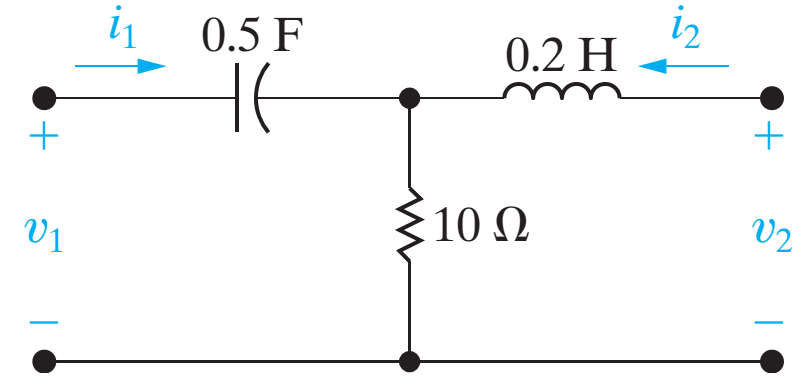
\includegraphics[width=\maxwidth{50.48670346211741em}]{image_0}
\end{flushleft}
\end{par}

\begin{enumerate}
\setlength{\itemsep}{-1ex}
   \item{\begin{flushleft} $z_{11}$ is the impedance seen looking into port 1 when port 2 is open. \end{flushleft}}
   \item{\begin{flushleft} $z_{12}$ is a transfer impedance. It is the ratio of the port 1 voltage to the port 2 current when port 1 is open. \end{flushleft}}
   \item{\begin{flushleft} $z_{21}$ is a transfer impedance. It is the ratio of the port 2 voltage to the port 1 current when port 2 is open. \end{flushleft}}
   \item{\begin{flushleft} $z_{22}$ is the impedance seen looking into port 2 when port 1 is open. \end{flushleft}}
\end{enumerate}

\begin{matlabcode}
syms s
z11 = (10 + 1/(0.5*s))*u.Ohm
\end{matlabcode}
\begin{matlabsymbolicoutput}
z11 = 
    $\displaystyle {\left(\frac{2}{s}+10\right)} {\Omega }$
\end{matlabsymbolicoutput}
\begin{matlabcode}
z21 = 10*u.Ohm
\end{matlabcode}
\begin{matlabsymbolicoutput}
z21 = 
    $\displaystyle 10 {\Omega }$
\end{matlabsymbolicoutput}
\begin{matlabcode}
z12 = 10*u.Ohm
\end{matlabcode}
\begin{matlabsymbolicoutput}
z12 = 
    $\displaystyle 10 {\Omega }$
\end{matlabsymbolicoutput}
\begin{matlabcode}
z22 = (0.2*s+10)*u.Ohm
\end{matlabcode}
\begin{matlabsymbolicoutput}
z22 = 
    $\displaystyle {\left(\frac{s}{5}+10\right)} {\Omega }$
\end{matlabsymbolicoutput}
\label{H_0DA4DB58}
\matlabheading{Problem 2 --- 19.26 Alexander sixth edition}

\begin{par}
\begin{flushleft}
19.26 Calculate [y] for the two-port in Fig. 19.85.
\end{flushleft}
\end{par}

\begin{par}
\begin{flushleft}
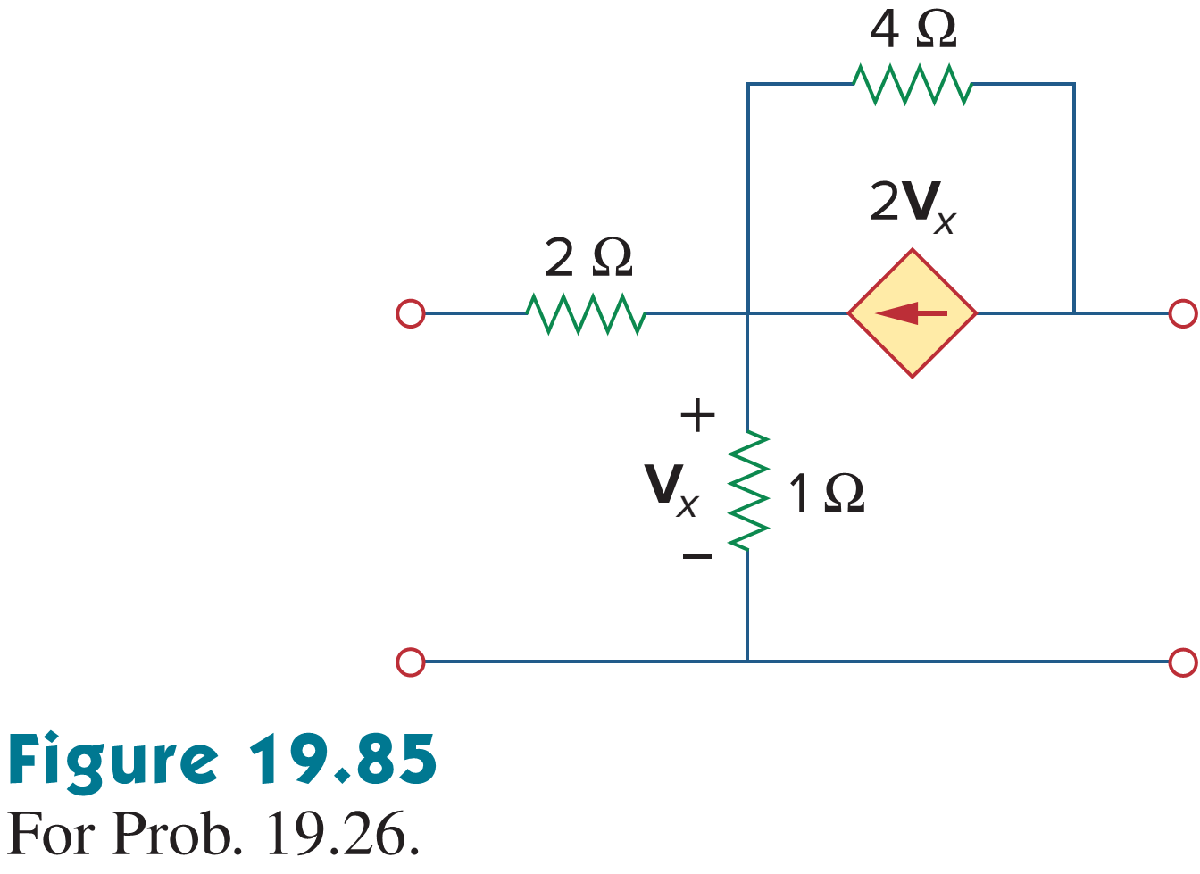
\includegraphics[width=\maxwidth{50.57701956848972em}]{image_1}
\end{flushleft}
\end{par}

\begin{par}
$$y_{11}= \frac{I_1}{V_1} \vert_{V_2=0} S, \quad \linebreak 
y_{21}= \frac{I_2}{V_1} \vert_{V_2=0} S,$$
\end{par}

\begin{par}
$$y_{12} = \frac{I_1}{V_2} \vert_{V_1=0} \ S, \quad\linebreak 
y_{22} = \frac{I_2}{V_2} \vert_{V_1=0} \ S$$
\end{par}

\begin{par}
\begin{flushleft}
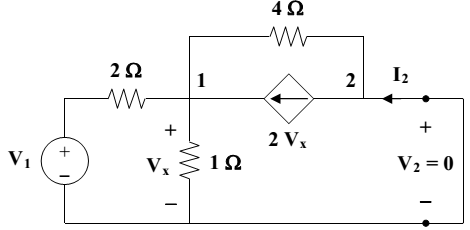
\includegraphics[width=\maxwidth{47.16507777220271em}]{image_2}
\end{flushleft}
\end{par}

\begin{matlabcode}
%syms V1 Vx
%p3eqn1 = (V1-Vx)/x+2*Vx == Vx/1+Vx/4
%p3eqn2 = 
y = [1.5 0.5; ...
    -3.5 -1.5]
\end{matlabcode}
\label{H_061A270D}
\matlabheading{Problem 3 --- 18.37 Nillison Riddel 5th edition}

\begin{par}
\begin{flushleft}
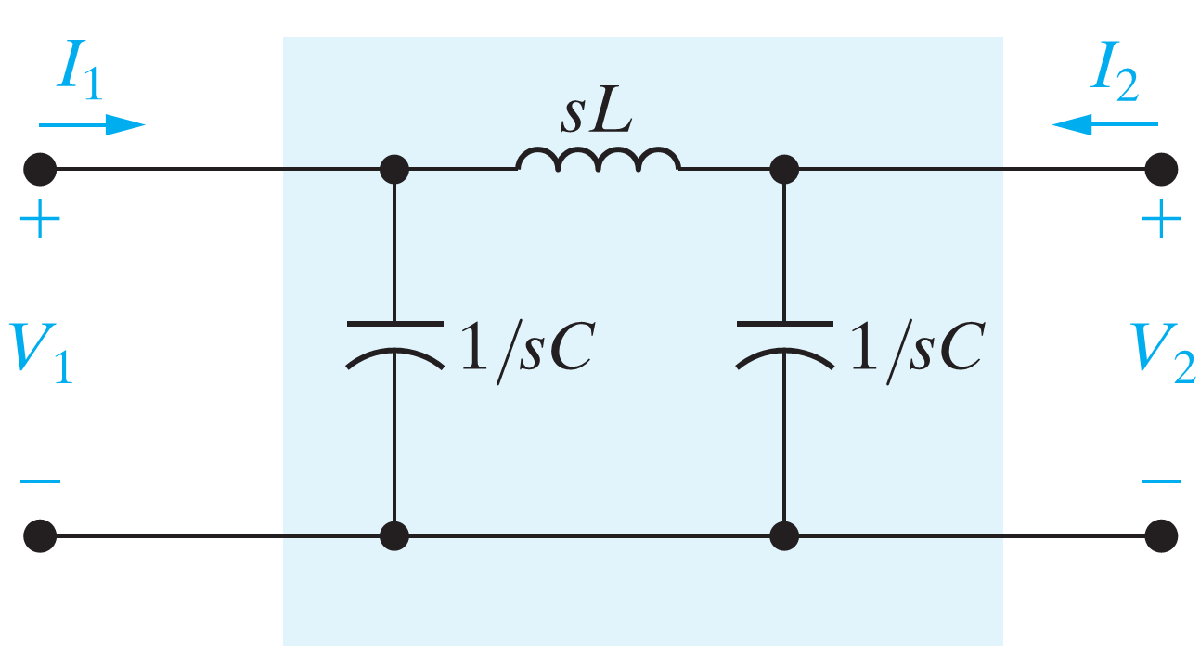
\includegraphics[width=\maxwidth{50.48670346211741em}]{image_3}
\end{flushleft}
\end{par}

\begin{par}
\begin{flushleft}
Find the \textit{s}-domain expressions for the \textit{g }parameters of the circuit in Fig. P18.37. Port 2 in Fig. P18.37 is terminated in a resistance of $500 \Omega$ and port 1 is driven by a step voltage source $v_1(t)=4u(t) V.$ Find $v_2(t)$ for $t > 0$ if C = 32 nF and L = 50 mH.
\end{flushleft}
\end{par}

\begin{par}
$$g_{11}= \frac{I_1}{V_1} \vert_{I_2=0} \ S, \quad\linebreak 
g_{12}= \frac{I_1}{I_2} \vert_{V_1=0}, $$
\end{par}

\begin{par}
$$g_{21}= \frac{V_2}{V_1} \vert_{I_2=0}, \quad\linebreak 
g_{22}= \frac{V_2}{I_2} \vert_{V_1=0} \quad \Omega$$
\end{par}

\begin{matlabcode}
syms C L
% Find g11
p3z111 = s*L+1/(s*C)
\end{matlabcode}
\begin{matlabsymbolicoutput}
p3z111 = 
    $\displaystyle L s+\frac{1}{C s}$
\end{matlabsymbolicoutput}
\begin{matlabcode}
p3z11 = (1/(s*C)*p3z111)/(1/(s*C)+p3z111)
\end{matlabcode}
\begin{matlabsymbolicoutput}
p3z11 = 
    $\displaystyle \frac{L s+\frac{1}{C s}}{C s {\left(L s+\frac{2}{C s}\right)}}$
\end{matlabsymbolicoutput}
\begin{matlabcode}
p3z11 = simplify(p3z11)
\end{matlabcode}
\begin{matlabsymbolicoutput}
p3z11 = 
    $\displaystyle \frac{C L s^2 +1}{C s {\left(C L s^2 +2\right)}}$
\end{matlabsymbolicoutput}
\begin{matlabcode}
p3g11 = 1/p3z11
\end{matlabcode}
\begin{matlabsymbolicoutput}
p3g11 = 
    $\displaystyle \frac{C s {\left(C L s^2 +2\right)}}{C L s^2 +1}$
\end{matlabsymbolicoutput}
\begin{matlabcode}
p3g11 = simplify(p3g11)
\end{matlabcode}
\begin{matlabsymbolicoutput}
p3g11 = 
    $\displaystyle \frac{C s {\left(C L s^2 +2\right)}}{C L s^2 +1}$
\end{matlabsymbolicoutput}
\begin{matlabcode}
% factor(p3g11)

% Find g21
p3g21 = 1/(s*C)/(s*L+1/(s*C))
\end{matlabcode}
\begin{matlabsymbolicoutput}
p3g21 = 
    $\displaystyle \frac{1}{C s {\left(L s+\frac{1}{C s}\right)}}$
\end{matlabsymbolicoutput}
\begin{matlabcode}
p3g21 = simplify(p3g21)
\end{matlabcode}
\begin{matlabsymbolicoutput}
p3g21 = 
    $\displaystyle \frac{1}{C L s^2 +1}$
\end{matlabsymbolicoutput}
\begin{matlabcode}

% Find g12 
ZC = 1/(s*C)
\end{matlabcode}
\begin{matlabsymbolicoutput}
ZC = 
    $\displaystyle \frac{1}{C s}$
\end{matlabsymbolicoutput}
\begin{matlabcode}
ZL = s*L
\end{matlabcode}
\begin{matlabsymbolicoutput}
ZL = 
    $\displaystyle L s$
\end{matlabsymbolicoutput}
\begin{matlabcode}
ZT = ZC + ZL
\end{matlabcode}
\begin{matlabsymbolicoutput}
ZT = 
    $\displaystyle L s+\frac{1}{C s}$
\end{matlabsymbolicoutput}
\begin{matlabcode}
p3g12 = ZC/ZT% Using current divider 
\end{matlabcode}
\begin{matlabsymbolicoutput}
p3g12 = 
    $\displaystyle \frac{1}{C s {\left(L s+\frac{1}{C s}\right)}}$
\end{matlabsymbolicoutput}
\begin{matlabcode}
% I1 and I2, (ZT / Zx)^{-1} = Zx / ZT
% Find g22, using sL || 1/sC
p3g22 = ZL*ZC/(ZL+ZC)
\end{matlabcode}
\begin{matlabsymbolicoutput}
p3g22 = 
    $\displaystyle \frac{L}{C {\left(L s+\frac{1}{C s}\right)}}$
\end{matlabsymbolicoutput}
\begin{matlabcode}
p3g22 = simplify(p3g22)
\end{matlabcode}
\begin{matlabsymbolicoutput}
p3g22 = 
    $\displaystyle \frac{L s}{C L s^2 +1}$
\end{matlabsymbolicoutput}

\begin{par}
\begin{flushleft}
Problem 4 --- 19.70* Alexander sixth edition
\end{flushleft}
\end{par}

\begin{par}
\begin{flushleft}
Problem 5 --- 18.7 Nillison Riddel fifth edition
\end{flushleft}
\end{par}

\vspace{1em}

\begin{par}
\begin{flushleft}
18.7 Select the values of and in the circuit in Fig. P18.7 so that  $h_{11}= 4 \Omega$, $h_{12}= 0.8$,
\end{flushleft}
\end{par}

\begin{par}
$$h_{21}= -0/8 $$ and $$h_{22}=0.14 S$$
\end{par}

\begin{par}
\begin{flushleft}
Problem 6 --- 18.30 Nillision Riddel 5th edition 18.30 The g parameters for the two-port circuit in Fig. P18.30 are
\end{flushleft}
\end{par}
\label{H_C9D11E55}
\matlabheading{Testing}

\begin{matlabcode}
x = [1 2 3 4]'
\end{matlabcode}
\begin{matlaboutput}
x = 4x1    
     1
     2
     3
     4

\end{matlaboutput}
\begin{matlabcode}
y = [4 5 6 7]'
\end{matlabcode}
\begin{matlaboutput}
y = 4x1    
     4
     5
     6
     7

\end{matlaboutput}
\begin{matlabcode}
% I presume that the matlab people are working on
% matlab package that can interpret all the matlab commands
% when that happens that will be fairly good.
table(x,y)
\end{matlabcode}
\begin{matlabtableoutput}
{
\begin{tabular}{|c|c|c|}
\hline
\mlcell{ } & \mlcell{x} & \mlcell{y} \\ \hline
\mlcell{1} & \mlcell{1} & \mlcell{4} \\ \hline
\mlcell{2} & \mlcell{2} & \mlcell{5} \\ \hline
\mlcell{3} & \mlcell{3} & \mlcell{6} \\ \hline
\mlcell{4} & \mlcell{4} & \mlcell{7} \\ 
\hline
\end{tabular}
}
\end{matlabtableoutput}

\end{document}
